% Versión 2021
%
\begin{tcolorbox}{Conceptos b\'asicos del sistema \ac{ADF}}

  \begin{itemize}
  \item El \ac{ADF}, es uno de los sistemas de radio navegación mas
    antiguos, est\'a compuesto por un equipo llevado a bordo de la
    aeronave y otros en tierra.

  \item La funci\'on del ADF es indicar al piloto la direcci\'on en la
    cual se encuentra una \ac{NDB} sintonizada.

  \item La \ac{NDB} es la correspondiente radioayuda en tierra que se
    sintoniza, mientras que el ADF es el equipo a bordo de la
    aeronave. El ADF puede utilizar se\~nales de otras fuentes, como
    radioemisoras comerciales.

  \item A nivel mundial, se utiliza el ancho de banda entre 200 kHz y
    1750 kHz (aunque los l\'imites pueden variar un poco seg\'un el
    lugar). En Europa los NDB t\'ipicamente se encuentran en las
    sub-bandas 255-415 y 510-525 kHz.

  \item Este rango de frecuencias coloca al sistema en el dominio de la
    \ac{MF}, entre las  ondas ionosf\'ericas (o de
    cielo) y las ondas de tierra. Estas \'ultimas son capaces de llegar a
    largas distancias y sobrepasar obst\'aculos.

  \item La longitud de onda es bastante grande
    comparada con las dimensiones de una aeronave: f = 200 kHz -
    $\lambda = 1500$ m, y f = 1750 kHz - $\lambda = 171.429$ m.

  \item La se\~nal se emite en \ac{AM},envi\'andose la
    identificaci\'on de la estaci\'on NDB en c\'odigo Morse
    o m\'usica y sonidos en el caso de las radioemisoras comerciales.

  \item El alcance es de 25 a 100 NM (46,3 a 185,2 km), puede ser
    mayor, pero aparecen problemas.

  \item La intensidad de campo requerida es de 70 $\mu$Voltios/m, con
    S/N $>$ 15 dB.

  \item La precisi\'on media obtenida es de 3º a 5º en condiciones
    normales de operaci\'on.

  \item La polarizaci\'on es vertical con propagaci\'on horizontal.
  \end{itemize}

\end{tcolorbox}

\subsection{Antena de cuadro}
\label{sec:06.antena.de.cuadro}

La antena de cuadro (tambi\'en llamada antena loop), es una evoluci\'on de las antenas ``Adcock'' que consiste en dos antenas verticales aisladas conectadas en contrafase, ver Figura \ref{fig:antena.adcock}.

La antena de cuadro tiene las antenas verticales conectadas entre s\'i y est\'a hecha de varias vueltas de hilo conductor para mejorar sus propiedades de recepci\'on, como se muestra en la Figura \ref{fig:antena.cuadro}.

Las dos secciones verticales de la antena son las que reciben la se\~nal, son paralelas entre s\'i y est\'an conectadas en ``contrafase'', lo que significa que lo que reciben se resta entre s\'i y lo que sale es la diferencia.

\begin{figure}[!h]
  \centering
 \subfigure[Antena Adcock %\\ {\tiny Fuente:\url{http://www.flyingstart.ca/FlightTraining/preflight/antennae.html}}
	]{
	 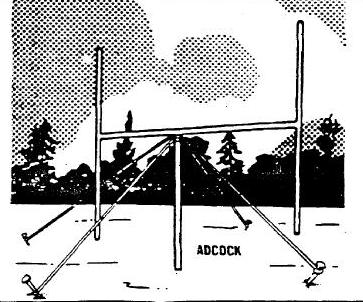
\includegraphics[width=0.4\textwidth]{06.radionavegacion/Imagenes/06.01.adf/adcock-antena-01.jpg}
	 \label{fig:antena.adcock}
	 }
% \subfigure[Antigua antena de cuadro ubicada en la parte baja del fuselaje de un DC3.\\ {\tiny Fuente:armyintelligence.tpub.com/IT0302/IT03020036.htm}]{\includegraphics[height=6.5cm]{Imagenes/06.01.adf/DC3-loop-antena.jpg}  \label{fig:antena.loop.vieja}}
 \subfigure[Antigua antena de cuadro ubicada en la parte baja del fuselaje de un DC3]{\includegraphics[width=0.4\textwidth]{06.radionavegacion/Imagenes/06.01.adf/DC3-loop-antena.jpg}  \label{fig:antena.loop.vieja}}
  \caption{Antenas}
\end{figure}




\subsection{Radiogoni\'ometro}

La evoluci\'on del ADF ha sido en fases. La primera de ellas fue el radiogoni\'ometro, que hallaba la direcci\'on en la cual se encontraba una estaci\'on emisora en tierra, pero NO lo hac\'ia de manera autom\'atica.

Este instrumento ten\'ia una antena de cuadro que pod\'ia girarse manualmente desde la cabina, como la mostrada en la Figura \ref{fig:antena.loop.vieja}.

El siguiente dibujo representa una antena de cuadro cuyo plano est\'a inclinado un cierto \'angulo $\theta$ con respecto al origen de la se\~nal:


\begin{figure}[!h]
  \centering
\subfigure[Antena de cuadro \protect\cite{ADF-teoria}]{  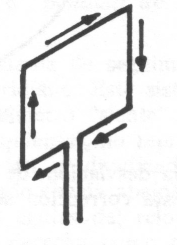
\includegraphics[width=0.3\textwidth]{06.radionavegacion/Imagenes/06.01.adf/antena-cuadro.png}  \label{fig:antena.cuadro}}
\subfigure[Recepci\'on de la se\~nal por la antena de cuadro \protect\cite{ADF-teoria}]{  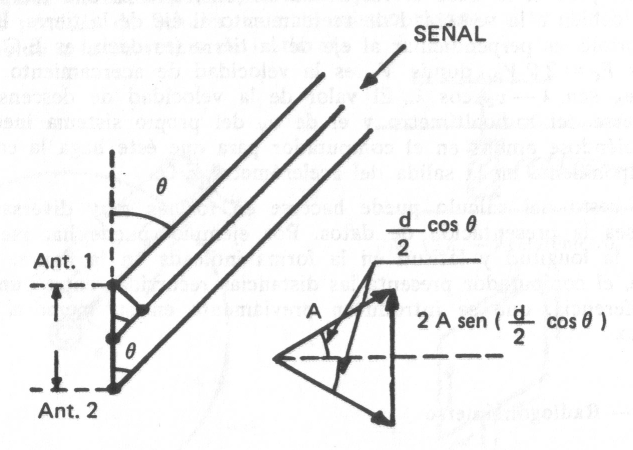
\includegraphics[width=0.6\textwidth]{06.radionavegacion/Imagenes/06.01.adf/antena-cuadro-recibiendo-senial.png}  \label{fig:antena.cuadro.recibiendo.senial}}
  \caption{Antena de cuadro}
\end{figure}


En la Figura \ref{fig:antena.cuadro.recibiendo.senial} se puede apreciar claramente que debido a que la ``Antena 1'' (Ant. 1 en la figura) y la ``Antena 2'' (Ant. 2) est\'an separadas una cierta distancia y, adem\'as, existe un \'angulo entre la se\~nal que llega y el plano que une las antenas ($\theta$), la primera recibe la se\~nal antes que la segunda. Por esto existe un desfase entre ambas, y por tanto una diferencia (la salida de la antena de cuadro NO es cero en este caso).

 En la Figura \ref{fig:seniales.recibidas.antena.cuadro} se ilustra la forma de las se\~nales recibidas por la antena 1 ($y_1$), la antena 2 ($y_2$) y la diferencia entre ellas ( $y_3 = y_2 - y_1$ ), que es realmente la salida de la antena de cuadro.

\begin{figure}[!h]
  \centering
  \subfigure[Se\~nales recibidas por la antena de cuadro ]{  \includegraphics[, height=6cm]{06.radionavegacion/Imagenes/06.01.adf/adf-seniales-antena-cuadro.eps}  \label{fig:seniales.recibidas.antena.cuadro}}
  \subfigure[Se\~nales recibidas por la antena de cuadro ]{  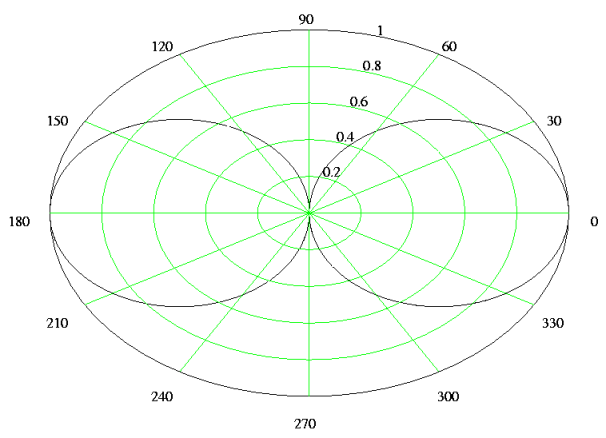
\includegraphics[height=6cm]{06.radionavegacion/Imagenes/06.01.adf/diagrama-recepcion-antena-cuadro.png}  \label{fig:diagrama.recepcion.antena.cuadro}}

  \caption{Esquemas funcionamiento antena de cuadro}
\end{figure}

En la Figura \ref{fig:diagrama.recepcion.antena.cuadro} se muestra un diagrama de recepci\'on de estas antenas, el resultado es una figura de ``ocho'', donde la recepci\'on es mayor cuando la se\~nal llega paralela al plano de la antena de cuadro, y nula cuando viene perpendicularmente.


Esta caracter\'istica es aprovechada para hallar la direcci\'on de donde proviene la se\~nal. El ``radionavegante'' a bordo del avi\'on ten\'ia en su panel de control una ruedecilla (acoplada a un indicador de direcci\'on) con la que pod\'ia girar a voluntad (y manualmente) la antena de cuadro, mientras simult\'aneamente escuchaba con sus aud\'ifonos la se\~nal de audio proveniente del emisor (NDB o estaci\'on de radio comercial).

Cuando el radionavegante dejaba de escuchar la se\~nal significaba que el plano de la antena de cuadro estaba perpendicular a la direcci\'on en la cual se encontraba el emisor, tomando nota de dicha direcci\'on (mostrada en el indicador) y marc\'andola en su carta de navegaci\'on.

El m\'etodo anterior encuentra la direcci\'on pero \emph{existe una ambigüedad en el sentido}, pues el emisor puede estar a un lado u otro del plano de la antena de cuadro. Esta ambigüedad era resuelta tomando otros emisores como referencia, y hallando la intersecci\'on de las direcciones, o llevando un registro cuidadoso de la trayectoria del avi\'on desde el inicio del vuelo.

En la Figura \ref{fig:diag-bloques-radiogoniometro} se ilustra el diagrama de bloques del radiogoni\'ometro.


\begin{figure}[!h]
  \centering
   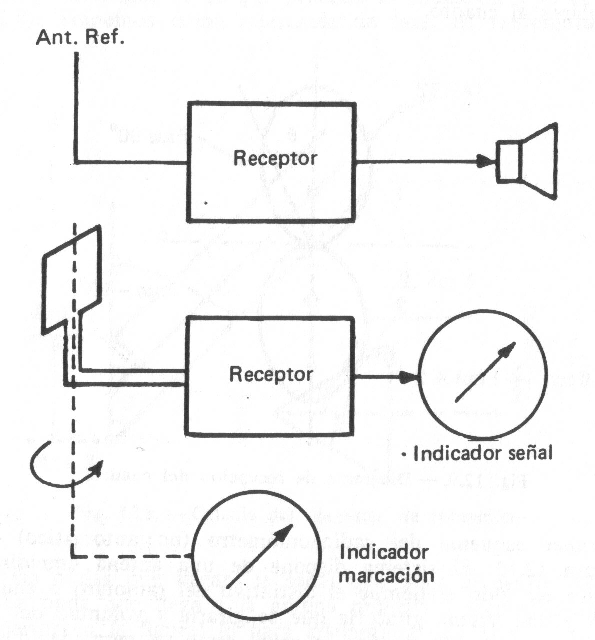
\includegraphics[width=0.5\textwidth]{06.radionavegacion/Imagenes/06.01.adf/diag-bloques-radiogoniometro.png}
  \caption{Diagrama de bloques del radiogoni\'ometro}
  \label{fig:diag-bloques-radiogoniometro}
\end{figure}


En un circuito aparte, alimentado por una ``\emph{antena de referencia}'', proporciona una se\~nal en el sistema de audio que no est\'a sometida a las variaciones de amplitud que implica el cambio de direcci\'on de la antena de cuadro.



\subsection{ADF}

La diferencia principal entre el radiogoni\'ometro y el ADF es que este \'ultimo es \emph{autom\'atico}, como lo indica su nombre. Esto indica que la ambigüedad en el sentido debe resolverse dentro del propio equipo.

Para ello, se instala una antena de referencia que, por comodidad, se representar\'a en el centro de la antena de cuadro. La se\~nal recibida por esta antena se considera que no tiene desfase y al graficarla en el tiempo ($y_4$) estar\'a entre $y_1$ y $y_2$, ver Figura \ref{fig:seniales-2}.


\begin{figure}[!h]
  \centering
  \subfigure[Se\~nales recibidas por la antena de cuadro + se\~nal de referencia. ]{  \includegraphics[width=0.45\textwidth]{06.radionavegacion/Imagenes/06.01.adf/adf-+seniales-antena-cuadro.eps}  \label{fig:seniales-2}}
  \subfigure[Se\~nales antena de cuadro + referencia + referencia desfasada 90º. ]{  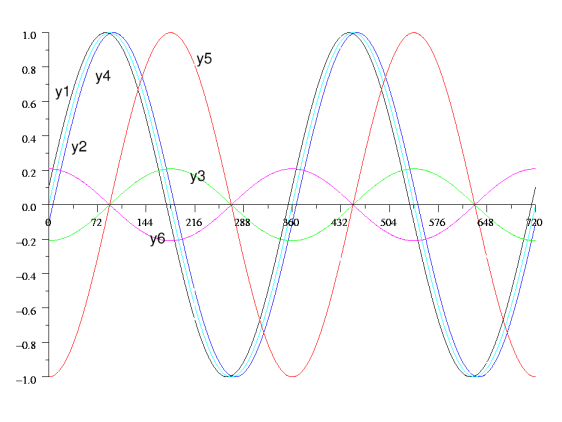
\includegraphics[width=0.45\textwidth]{06.radionavegacion/Imagenes/06.01.adf/senyales-3.png}  \label{fig:seniales-3}}

  \subfigure[Diagrama de recepci\'on antena de cuadro + antena de referencia.]{  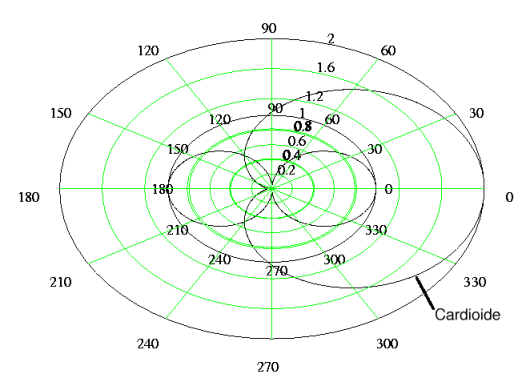
\includegraphics[width=0.65\textwidth]{06.radionavegacion/Imagenes/06.01.adf/diag-recepcion-2.png}  \label{fig:diag-recepcion-2}}

  \caption{Se\~nales recibidas por la antena de cuadro}
\end{figure}


Si la se\~nal de referencia se desfasa 90º (en la Figura \ref{fig:seniales-3} se indica como curva $y_5$), se puede apreciar que pr\'acticamente entra en fase con $y_3$, la cual es la salida de la antena de cuadro cuando la antena 1 est\'a m\'as cerca del emisor que la antena 2. Correspondientemente, $y_5$ estar\'a en contrafase con $y_3$ si es la antena 2 la que est\'a m\'as cerca del emisor ($y_6 = y_1 - y_2$). %Lo anterior se representa en la Figura \ref{fig:seniales-3}. 

Esta caracter\'istica de la recepci\'on se aprovecha para determinar el sentido en el que se encuentra el sector y as\'i resolver la ambigüedad que padec\'ia el radiogoni\'ometro. Si se hace un diagrama de recepci\'on de la combinaci\'on antena de cuadro + antena de referencia, se obtiene un diagrama de radiaci\'on en forma de curva \emph{cardioide}, ver Figura \ref{fig:diag-recepcion-2}.


Entonces, la se\~nal de la antena de cuadro es introducida alternativamente a dos combinadores que generan 2 cardioides: Uno recibe $y_3$ ($y_2-y_1$) y el otro $y_6$ ($y_1-y_2$). \'Estos a su vez tambi\'en reciben $y_5$ y la salida de ambos alimenta a un comparador.

El resultado de la comparaci\'on es amplificado y alimenta a su vez al motor que mueve el cuadro. Este motor girar\'a en un sentido u otro seg\'un el signo de la comparaci\'on dejando de mover la antena cuando la se\~nal de ambas cardioides resulte igual. Un acoplador selsyn conectado al motor del cuadro transmite la se\~nal hasta un indicador en la cabina de vuelo.

En la Figura \ref{fig:diag-bloques-adf-rot} se presenta el diagrama de bloques de lo anterior.

% \begin{figure}[!h]
%   \centering
%   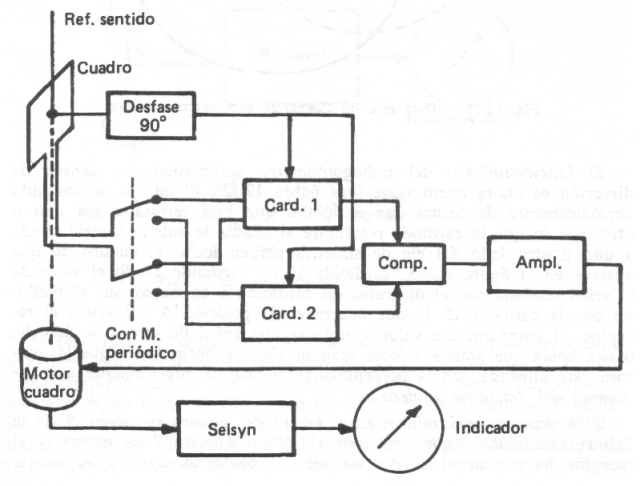
\includegraphics[width=0.75\textwidth]{06.radionavegacion/Imagenes/06.01.adf/diag-bloques-adf-rot.png}   
%   \label{fig:diag-bloques-adf-rot}
%   \caption{Diagrama  de bloques del ADF con antena rotatoria}
% \end{figure}


%\begin{landscape}
 
 \begin{figure}[!h]
    \centering \subfigure[Diagrama de bloques del ADF con antena
    rotatoria]{ 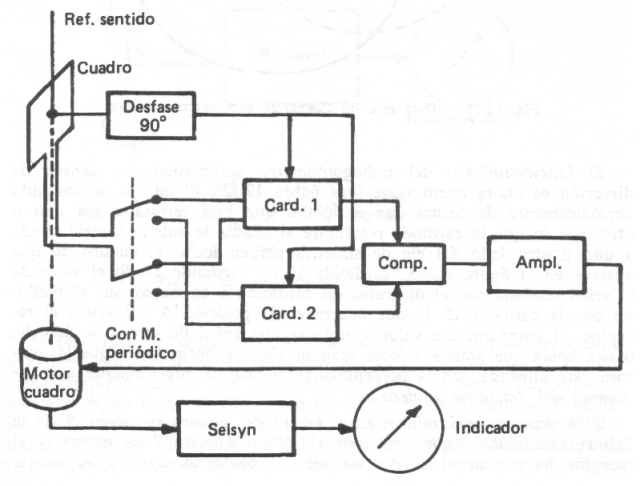
\includegraphics[width=0.45\textwidth]{06.radionavegacion/Imagenes/06.01.adf/diag-bloques-adf-rot.png} \label{fig:diag-bloques-adf-rot}}
    \subfigure[Diagrama de bloques del ADF con antena
    rotatoria]{ 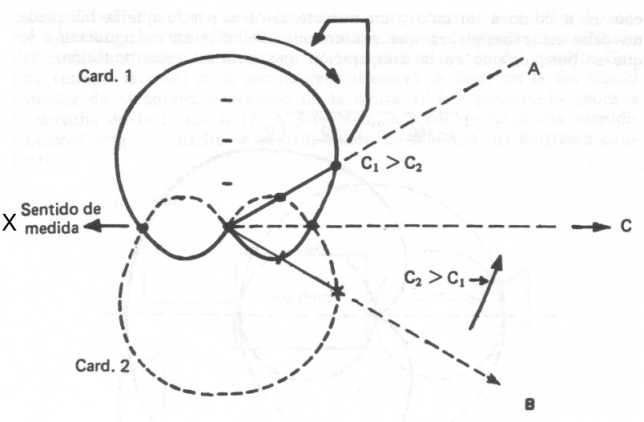
\includegraphics[width=0.45\textwidth]{06.radionavegacion/Imagenes/06.01.adf/esquema-adf-rot.png} \label{fig:esquema-adf-rot}}
    \caption{}
  \end{figure}


%\end{landscape}

El siguiente esquema muestra las cardioides que el comparador est\'a recibiendo de los combinadores y c\'omo el sistema reacciona seg\'un cada caso, ver Figura \ref{fig:esquema-adf-rot}.

%\subsubsection{Reacciones del sistema ADF con antena rotatoria}

Para explicar estas reacciones vamos a estudiarlas por casos, siempre teniendo en cuenta que la flecha denotada como ``\emph{Sentido de la medida}'' representa la flecha del indicador:

\begin{description}
\item[\bf Emisor en posici\'on A:] En este caso, la cardioide 1 ($C_11$) es mayor que la cardioide 2 ($C_2$), $C_1 > C_2$ lo que hace que el comparador emita una se\~nal al motor del cuadro que har\'a rotar al conjunto COMO LAS AGUJAS DEL RELOJ (unos 150º en este caso) hasta que la flecha apunte hacia ``A''. Cuando se llegue a ese punto, $C_1=C_2$ y se detendr\'a el movimiento.


\item[\bf Emisor en posici\'on B:] Ahora el comparador hallar\'a que $C_2 > C_1$, y por tanto dar\'a al motor del cuadro la orden de giro AL CONTRARIO DE LAS AGUJAS DEL RELOJ hasta que la flecha apunte hacia ``\emph{B}'', lugar en donde se detiene el giro porque $C_1 = C_2$.
    

\item[\bf Emisor en posici\'on X:] En este caso no hay movimiento porque la estaci\'on est\'a precisamente en donde $C_1 = C_2$. No obstante, si por alguna desviaci\'on de la aeronave resulta que la flecha apuntara brevemente un poco ``\emph{por debajo}'' de ``\emph{X}'', entonces $C_1 > C_2$ y el motor empezar\'a a girar como las agujas del reloj, lo que posicionar\'a la flecha otra vez en ``X''. Si por el contrario la flecha apuntara brevemente ``\emph{por encima}'' de ``\emph{X}'', entonces $C_2 > C_1$ y el motor girar\'ia al rev\'es del reloj, volviendo a colocar la flecha apuntando a ``\emph{X}''. En definitiva, esta posici\'on es de equilibrio estable.


\item[\bf Emisor en posici\'on C:] Esta posici\'on representa aparentemente un problema porque la estaci\'on est\'a situada justamente al contrario de lo indicado por la flecha, pero como $C_1 = C_2$ en teor\'ia la aguja permanecer\'ia en la posici\'on err\'onea. Sin embargo, la m\'as ligera desviaci\'on de esta posici\'on provocar\'ia que el conjunto diera una vuelta de 180º, colocando a la flecha en la posici\'on correcta. Por ejemplo, si C se mueve relativamente un poco hacia abajo de abajo de la posici\'on actual, $C_2 > C_1$ y la antena se mover\'ia al contrario del reloj, aumentando a cada momento la diferencia entre $C_2$ y $C_1$, hasta que se d\'e una vuelta completa y se encuentre de nuevo el equilibrio, ahora con la flecha apuntando en el sentido correcto. Por tanto, la posici\'on ``C'' es de ``\emph{equilibrio inestable}'' y no representa un problema en la pr\'actica.
 
\end{description}
    

Conforme evolucion\'o la tecnolog\'ia, se encontraron maneras de desarrollar un sistema ADF que resolviera la ambigüedad de sentido sin necesidad de rotar la antena de cuadro, mejor\'andose la confiabilidad del sistema.

Para ello, se utilizan dos antenas de cuadro colocadas ortogonalmente. La que tiene su plano a lo largo del eje longitudinal del avi\'on (adelante-atr\'as) es la ``\textbf{antena coseno}'', mientras aquella cuyo plano coincide con el eje transversal es la ``\textbf{antena seno}'', ver Figura \ref{fig:esquema-adf-fijo}.

De esta manera se tienen dos diagramas de recepci\'on en ``\emph{ocho}'', perpendiculares entre s\'i, que generar\'an sus respectivas cardioides al ser adecuadamente combinados con la se\~nal proveniente de la antena de referencia.% Observe el siguiente diagrama:



De forma an\'aloga al caso del ADF con antena rotatoria, las se\~nales provenientes de las antenas de cuadro son combinadas con la se\~nal de la antena de referencia y alimentan alternativamente (con una frecuencia de alternancia de 100 Hz) a un comparador de fases. La salida de \'este son los valores de seno y coseno del \'angulo $\theta$ entre el eje longitudinal del avi\'on y la posici\'on de la estaci\'on.

Estas se\~nales seno-coseno alimentan a los indicadores (por ejemplo, un Indicador Radio-Magn\'etico o RMI), o a trav\'es de una interfaz ARINC 429 a un bus de datos digital.

En la Figura \ref{fig:diag-bloques-adf-fijo} se encuentra el diagrama de bloques t\'ipico de este sistema.

\begin{figure}[!h]
  \centering
  \subfigure[Diagrama de las antenas de cuadro ortogonales]{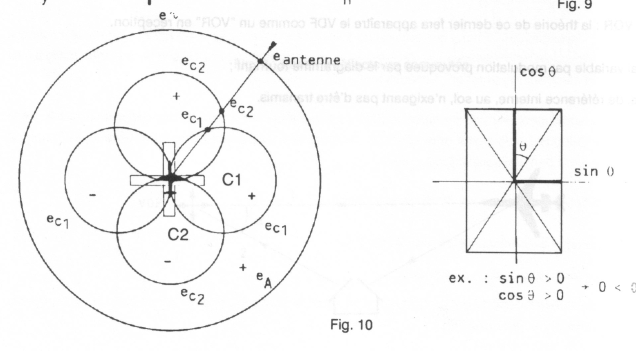
\includegraphics[width=0.75\textwidth]{06.radionavegacion/Imagenes/06.01.adf/esquema-adf-fijo.png}\label{fig:esquema-adf-fijo}}
  \subfigure[Diagrama de bloques del ADF con antenas fijas]{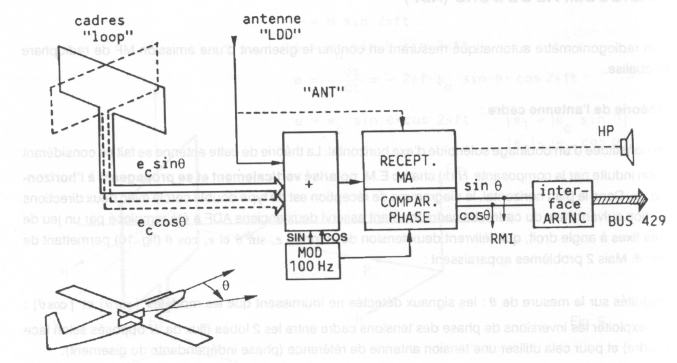
\includegraphics[width=0.75\textwidth]{06.radionavegacion/Imagenes/06.01.adf/diag-bloques-adf-fijo.png}\label{fig:diag-bloques-adf-fijo}}
  \caption{ADF fijo}
\end{figure}

\Informacion{Antenas para ADF}{
En el \href{https://www.sensorantennas.com/product/adf-antenna/}{siguiente link} puede accederse a una antena ADF comercial.

\href{http://verdanttelemetry.com/products-list.php?prdtcat_id=148}{Otro link} con informaci\'on de antenas ADF.
}



\subsubsection{NDB}
Como se indic\'o previamente, el NDB es la radioayuda en tierra que corresponde al ADF. Las sub-bandas de frecuencia usadas en Europa para los NDB t\'ipicamente se encuentran entre 255-415 y 510-525 kHz. Los NDB modulan en AM su identificaci\'on de estaci\'on en c\'odigo Morse, compuesta usualmente por tres letras.

\begin{figure}[!h]
  \centering
  \subfigure[S\'imbolo NDB usado en cartas aeron\'auticas ]{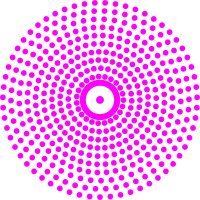
\includegraphics[width=0.15\textwidth]{06.radionavegacion/Imagenes/06.01.adf/NDB-simbolo.png}\label{fig:simbolo_ndb}} 
	\hspace{20pt}
  \subfigure[Emisor NDB en 49º 12.35' N, 2º 13.20' W. Callsign JW - 'Jersey West'. 329.0 kHz]{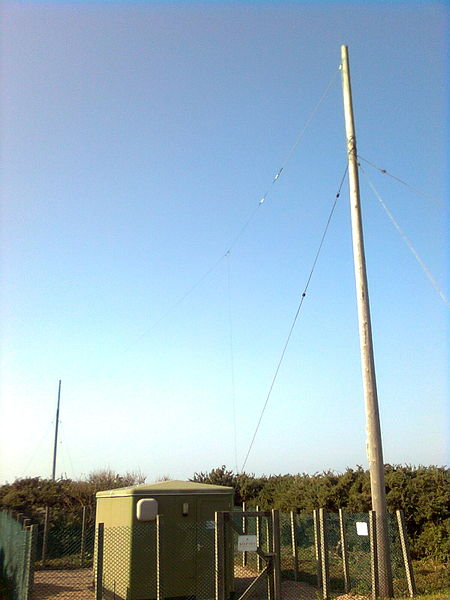
\includegraphics[width=0.25\textwidth]{06.radionavegacion/Imagenes/06.01.adf/NDB-transmisor.jpg}\label{fig:imagen_ndb}}
  \caption{NDB}
\end{figure}


Estos radiofaros con emisi\'on omnidirecciona en azimut tienen la caracter\'istica que sus antenas no pueden radiar en su direcci\'on longitudinal, por lo cual justo por encima de los NDBs se forma un cono en el cual NO existe se\~nal.

Este cono, caracter\'istico tambi\'en de otras radioayudas, es llamado ``cono de silencio'', y su \'angulo de abertura puede tener, en el caso de los NDB, hasta 45º.

El alcance de los NDB puede ir desde unas 25 NM ($\Resultado{1852 * 25}{0}$\,m) hasta m\'as de 100 NM, dependiendo de la potencia de emisi\'on. M\'as all\'a de las 100 NM empiezan a aparecer importantes errores.

\Informacion{Estaciones NDB en Argentina}{
Por el \href{http://186.153.175.229/descarga/aip-5b6deb26b09dd}{siguiente link} puede accederse a una lista de las estaciones NDB y otras radioayudas disponibles en Argentina en el a\~no 2018.
}

%\begin{landscape}
  \subsubsection{Presentaci\'on de la informaci\'on}
  \label{sec:06.adf.presentacion.informacion}

  % \url{https://greatbustardsflight.blogspot.com/2019/09/indicador-de-direccion-df-direction.html}

  % \begin{figure}[!h]
  %   \centering
  %   \subfigure[RBI]{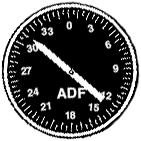
\includegraphics[width=0.3\textwidth]{06.radionavegacion/Imagenes/06.01.adf/RBI-0001.jpg}}
  %   \subfigure[RBI]{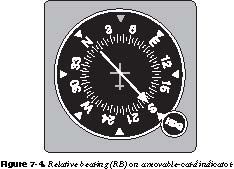
\includegraphics[width=0.4\textwidth]{06.radionavegacion/Imagenes/06.01.adf/RMI.jpg}}
  %   \subfigure[RMI +
  %   VOR]{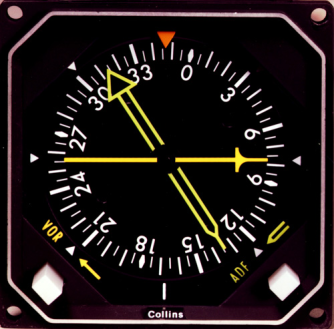
\includegraphics[width=0.25\textwidth]{06.radionavegacion/Imagenes/06.01.adf/rmi-adf-vor.png}}
  %   \caption{Formas de presentaci\'on de la informaci\'on}
  %   \label{fig:06.RBI.RMI}
  % \end{figure}

La informaci\'on presentada al piloto puede ser en forma de \ac{RBI} (Figura \ref{fig:06.RBI}) o como \ac{RMI} (Figura \ref{fig:06.RMI}), donde tambi\'en se presenta el QDM (rumbo magn\'etico a una estaci\'on),ver Figura  \ref{fig:06.QDM}. 

\begin{figure}[!h]
  \centering
  \subfigure[ADF]{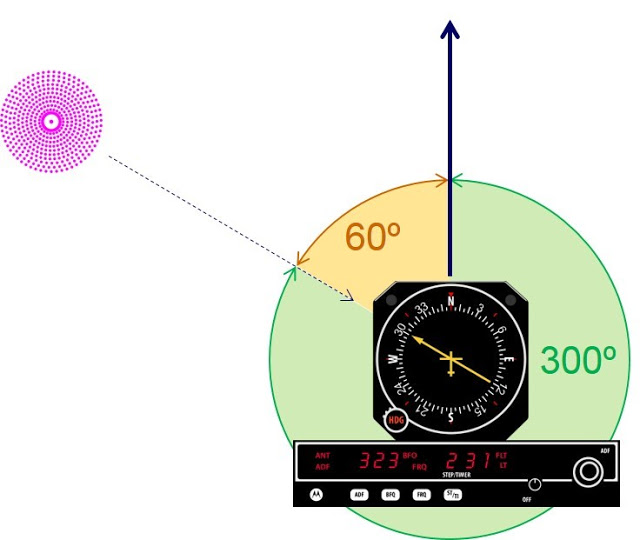
\includegraphics[width=0.4\textwidth]{06.radionavegacion/Imagenes/06.01.adf/adf-1.jpg} \label{fig:06.RBI}}
  \subfigure[QDM]{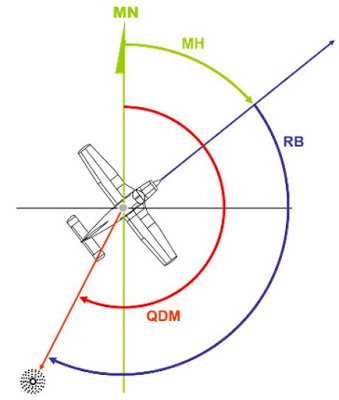
\includegraphics[width=0.25\textwidth]{06.radionavegacion/Imagenes/06.01.adf/QDM.jpg} \label{fig:06.QDM}}

  \subfigure[ADF]{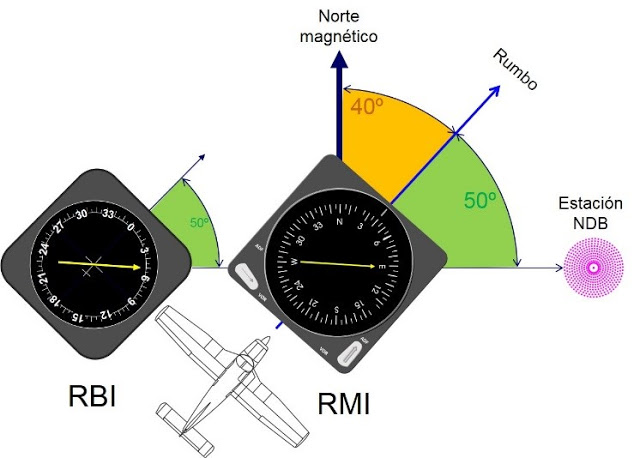
\includegraphics[width=0.6\textwidth]{06.radionavegacion/Imagenes/06.01.adf/adf-2.jpg} \label{fig:06.RMI}}
  \caption{Formas de presentaci\'on de la informaci\'on \protect\cite{QDM-RBI-RMI}}
  \label{fig:06.RBI.RMI}
\end{figure}

%\end{landscape}



\subsubsection{Errores ADF-NDB}

El sistema ADF/NDB tiene errores que t\'ipicamente oscilan entre los 3º y 5º. Hay dos tipos principales de error que son:

\begin{description}
\item [Errores Sistem\'aticos]

Los errores sistem\'aticos se pueden caracterizar previamente y tomar previsiones ante ellos. Los m\'as importantes son:

\begin{description}
\item [Error Instrumental]

Es el error asociado a incertidumbres en la lectura de los valores mostrados por los instrumentos. Oscila de 1 a 2 grados.

\item [Error por presencia del avi\'on]

La aeronave es un cuerpo met\'alico que puede interferir con la recepci\'on del sistema, distorsionando las se\~nales. Sin embargo, este error puede caracterizarse de f\'abrica y entonces tomar medidas correctivas.

\end{description}


\item [Errores Variables]

Como su nombre lo indica, son errores cuya aparici\'on y magnitud depende de m\'ultiples factores, siendo esencialmente desconocidos. Los m\'as conocidos son:

\begin{description}

\item [Errores atmosf\'ericos (tormentas)]

El n\'ucleo de las grandes tormentas genera poderosas cargas electromagn\'eticas cuya frecuencia puede estar en la banda de trabajo del ADF. Esto ocasiona que las tormentas puedan aparecer como estaciones en tierra y el ADF apuntar\'a hacia ellas. Es muy peligroso que el piloto las confunda con estaciones reales y vuele hacia ellas.


\item [Errores de polarizaci\'on]

Ciertas condiciones pueden alterar la polarizaci\'on y propagaci\'on de las se\~nales y ocasionar errores. Las m\'as conocidas son:

\begin{description}
\item [Efecto de l\'inea de costa], causado por la diferente conductividad entre la corteza terrestre y el agua, ocasionando que la se\~nal se refracte al pasar por la costa y genere indicaciones erradas.


\item [Efecto monta\~na], en donde debido a la orograf\'ia las ondas de tierra se pueden distorsionar, apareciendo errores de medici\'on.

\end{description}


\item [Interferencia xDSL (en estudio)]

La transmisi\'on de datos por Internet utilizando la tecnolog\'ia xDSL (HDSL, SDSL, VDSL y ADSL) puede generar se\~nales que interfieran con la operaci\'on del ADF y con las comunicaciones HF.

Debido a la naturaleza de los sistemas xDSL la fuente de interferencia est\'a distribuida geogr\'aficamente. Se est\'an realizando estudios para determinar si el efecto acumulativo de muchas de estas se\~nales puede alterar seriamente el funcionamiento del sistema (referencia actualizada al 21/Sep/2000).


\item [Efecto FADING]

Este efecto de ``desvanecimiento'' aparece porque a cierta distancia de la estaci\'on emisora las ``ondas de suelo'' y las ``ondas de cielo'' (estas \'ultimas por rebote ionosf\'erico) empiezan a interferir entre s\'i.
\vspace{10pt}

\begin{minipage}[b]{0.5\linewidth}
La interferencia entre ambas se\~nales puede ser constructiva o destructiva seg\'un el desfase que exista entre ellas, produci\'endose el efecto de una recepci\'on err\'atica e intermitente.

El siguiente gr\'afico representa la intensidad de campo versus la distancia a la estaci\'on, indicando las zonas en donde es m\'as probable que ocurra este efecto.
Una observaci\'on final es que durante la noche y cuando la aeronave se aproxima al ``terminator'' (l\'inea divisoria entre el d\'ia y la noche) es m\'as probable que se produzca este efecto, debido a la variaci\'on en la altura de la ionosfera.

\end{minipage}
\begin{minipage}[b]{0.5\linewidth}
  % \begin{figure}[!htb]
  \centering
  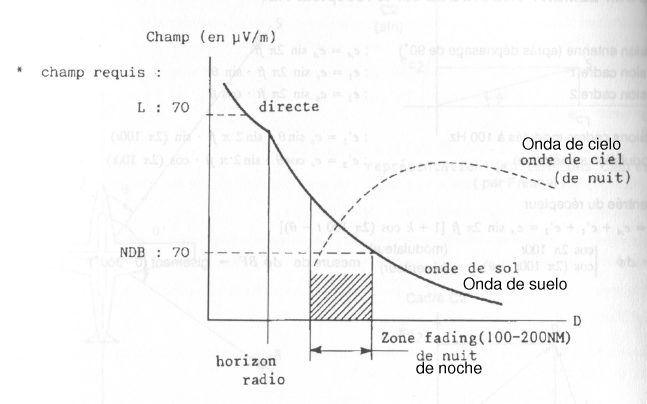
\includegraphics[width=\linewidth]{06.radionavegacion/Imagenes/06.01.adf/grafico-fading.png}
%  \captionof{ Gr\'afico del efecto ``fading''}
  \label{fig:fading}
%\end{figure}  
\end{minipage}





\end{description}

\end{description}


